\chapter{Psalm 15}

\begin{figure}
  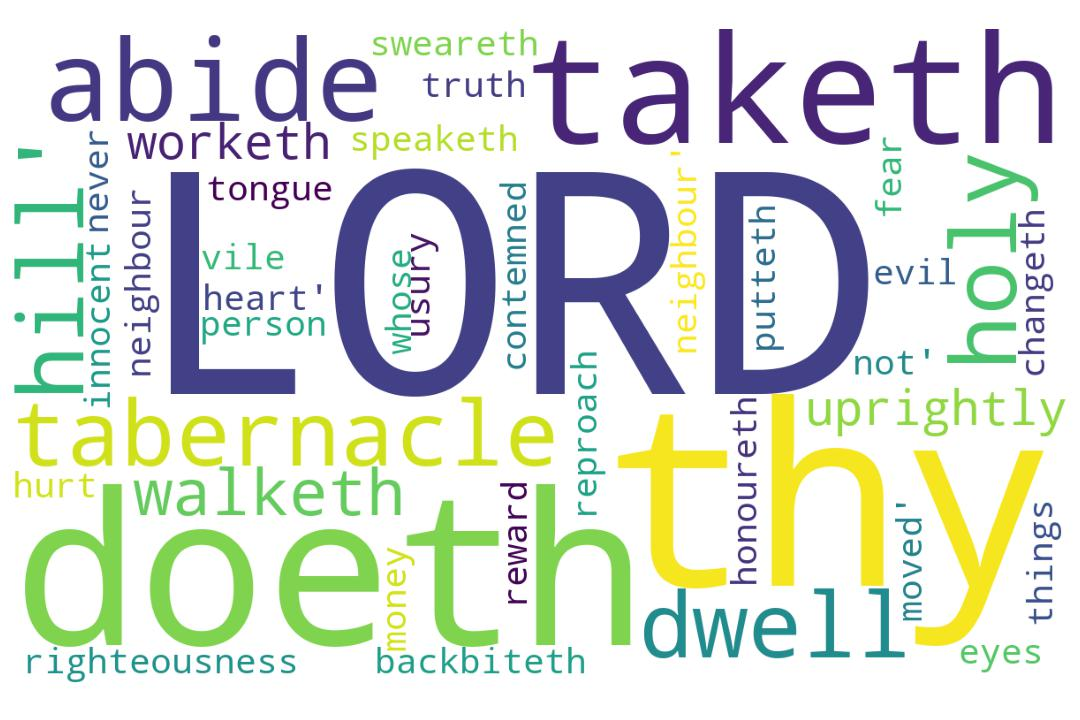
\includegraphics[width=\linewidth]{19OT-Psalms/Psalm15-WordCloud.jpg}
  \caption{Psalm 15 Word Cloud}
  \label{fig:Psalm 15 word Cloud}
\end{figure}



\marginpar{\scriptsize \centering \fcolorbox{bone}{lime}{\textbf{WHO DWELLS WITH GOD}}\\ (Psalm 15:1--5) \begin{compactenum}[I.][8]
    \item He who \textbf{Works Righteousness} \index[scripture]{Psalms!Psa 015:02} (Psa 15:2)
    \item He who \textbf{Meditates on Truth} \index[scripture]{Psalms!Psa 015:02} (Psa 15:2)
    \item He who \textbf{Does Not Backbite in Speech} -  (\index[scripture]{Psalms!Psa 015:03}Psa 15:3)
    \item He who \textbf{Treats his Neighbour Well} \index[scripture]{Psalms!Psa 015:03} \index[scripture]{Psalms!Psa 012:02} \index[scripture]{Psalms!Psa 101:05} (Psa 12:22, 15:3, and 101:5)
    \item He whose \textbf{Eyes Despise a Vile Man} \index[scripture]{Psalms!Psa 015:04} (Psa 15:4)
    \item He who \textbf{Does Not Put his Money Out to Usury} \index[scripture]{Psalms!Psa 015:05} (Psa 15:5) 
    \item He who \textbf{Does Not Betray the Brethren} \index[scripture]{Psalms!Psa 015:05} (Psa 15:5) 
\end{compactenum}}


\marginpar{\scriptsize \centering \fcolorbox{bone}{yellow}{\textbf{THE EVALUATION}}\\ (Psalm 15:1--5) \begin{compactenum}[I.][8]
    \item The \textbf{Everyday} Decisions 
    \item The \textbf{Eviction} Notice
    \item The \textbf{Event(s)} 
    \item The \textbf{Evidence} 
    \item The \textbf{Evil} Shunned and Avoided
    \item The \textbf{Evasion} from the Wicked
    \item The \textbf{Evaluation} 
\end{compactenum}}



\footnote{\textcolor[cmyk]{0.99998,1,0,0}{\hyperlink{TOC}{Return to end of Table of Contents.}}}\footnote{\href{https://www.audioverse.org/english/audiobibles/books/ENGKJV/O/Ps/1}{\textcolor[cmyk]{0.99998,1,0,0}{Psalms Audio}}}\textcolor[cmyk]{0.99998,1,0,0}{A Psalm of David.}\\
\\
\textcolor[cmyk]{0.99998,1,0,0}{LORD, who shall abide in thy tabernacle? who shall dwell in thy holy hill?}
[2] \textcolor[cmyk]{0.99998,1,0,0}{He that walketh uprightly, and \fcolorbox{bone}{lime}{worketh righteousness}, and \fcolorbox{bone}{lime}{speaketh the} \fcolorbox{bone}{lime}{truth in his} \fcolorbox{bone}{lime}{heart}.}
[3] \textcolor[cmyk]{0.99998,1,0,0}{\emph{He} \emph{that} \fcolorbox{bone}{lime}{backbiteth not} with his tongue, \fcolorbox{bone}{lime}{nor doeth} \fcolorbox{bone}{lime}{evil to his neighbour}, nor taketh up a reproach against his neighbour.}
[4] \textcolor[cmyk]{0.99998,1,0,0}{In whose eyes \fcolorbox{bone}{lime}{a vile person is} \fcolorbox{bone}{lime}{contemned}; but he honoureth them that fear the LORD. \emph{He} \emph{that} sweareth to \emph{his} \emph{own} hurt, and changeth not.}
[5] \textcolor[cmyk]{0.99998,1,0,0}{\emph{He} \emph{that} \fcolorbox{bone}{lime}{putteth not out his money} to usury, \fcolorbox{bone}{lime}{nor taketh reward} against the innocent. He that doeth these \emph{things} shall never be moved.}